% Options for packages loaded elsewhere
\PassOptionsToPackage{unicode}{hyperref}
\PassOptionsToPackage{hyphens}{url}
\PassOptionsToPackage{dvipsnames,svgnames,x11names}{xcolor}
%
\documentclass[
  letterpaper,
  DIV=11,
  numbers=noendperiod]{scrartcl}

\usepackage{amsmath,amssymb}
\usepackage{setspace}
\usepackage{iftex}
\ifPDFTeX
  \usepackage[T1]{fontenc}
  \usepackage[utf8]{inputenc}
  \usepackage{textcomp} % provide euro and other symbols
\else % if luatex or xetex
  \usepackage{unicode-math}
  \defaultfontfeatures{Scale=MatchLowercase}
  \defaultfontfeatures[\rmfamily]{Ligatures=TeX,Scale=1}
\fi
\usepackage{lmodern}
\ifPDFTeX\else  
    % xetex/luatex font selection
\fi
% Use upquote if available, for straight quotes in verbatim environments
\IfFileExists{upquote.sty}{\usepackage{upquote}}{}
\IfFileExists{microtype.sty}{% use microtype if available
  \usepackage[]{microtype}
  \UseMicrotypeSet[protrusion]{basicmath} % disable protrusion for tt fonts
}{}
\makeatletter
\@ifundefined{KOMAClassName}{% if non-KOMA class
  \IfFileExists{parskip.sty}{%
    \usepackage{parskip}
  }{% else
    \setlength{\parindent}{0pt}
    \setlength{\parskip}{6pt plus 2pt minus 1pt}}
}{% if KOMA class
  \KOMAoptions{parskip=half}}
\makeatother
\usepackage{xcolor}
\setlength{\emergencystretch}{3em} % prevent overfull lines
\setcounter{secnumdepth}{-\maxdimen} % remove section numbering
% Make \paragraph and \subparagraph free-standing
\ifx\paragraph\undefined\else
  \let\oldparagraph\paragraph
  \renewcommand{\paragraph}[1]{\oldparagraph{#1}\mbox{}}
\fi
\ifx\subparagraph\undefined\else
  \let\oldsubparagraph\subparagraph
  \renewcommand{\subparagraph}[1]{\oldsubparagraph{#1}\mbox{}}
\fi


\providecommand{\tightlist}{%
  \setlength{\itemsep}{0pt}\setlength{\parskip}{0pt}}\usepackage{longtable,booktabs,array}
\usepackage{calc} % for calculating minipage widths
% Correct order of tables after \paragraph or \subparagraph
\usepackage{etoolbox}
\makeatletter
\patchcmd\longtable{\par}{\if@noskipsec\mbox{}\fi\par}{}{}
\makeatother
% Allow footnotes in longtable head/foot
\IfFileExists{footnotehyper.sty}{\usepackage{footnotehyper}}{\usepackage{footnote}}
\makesavenoteenv{longtable}
\usepackage{graphicx}
\makeatletter
\def\maxwidth{\ifdim\Gin@nat@width>\linewidth\linewidth\else\Gin@nat@width\fi}
\def\maxheight{\ifdim\Gin@nat@height>\textheight\textheight\else\Gin@nat@height\fi}
\makeatother
% Scale images if necessary, so that they will not overflow the page
% margins by default, and it is still possible to overwrite the defaults
% using explicit options in \includegraphics[width, height, ...]{}
\setkeys{Gin}{width=\maxwidth,height=\maxheight,keepaspectratio}
% Set default figure placement to htbp
\makeatletter
\def\fps@figure{htbp}
\makeatother

\usepackage{booktabs}
\usepackage{longtable}
\usepackage{array}
\usepackage{multirow}
\usepackage{wrapfig}
\usepackage{float}
\usepackage{colortbl}
\usepackage{pdflscape}
\usepackage{tabu}
\usepackage{threeparttable}
\usepackage{threeparttablex}
\usepackage[normalem]{ulem}
\usepackage{makecell}
\usepackage{xcolor}
\usepackage{caption}
\usepackage{placeins}
\KOMAoption{captions}{tableheading}
\makeatletter
\makeatother
\makeatletter
\makeatother
\makeatletter
\@ifpackageloaded{caption}{}{\usepackage{caption}}
\AtBeginDocument{%
\ifdefined\contentsname
  \renewcommand*\contentsname{Table of contents}
\else
  \newcommand\contentsname{Table of contents}
\fi
\ifdefined\listfigurename
  \renewcommand*\listfigurename{List of Figures}
\else
  \newcommand\listfigurename{List of Figures}
\fi
\ifdefined\listtablename
  \renewcommand*\listtablename{List of Tables}
\else
  \newcommand\listtablename{List of Tables}
\fi
\ifdefined\figurename
  \renewcommand*\figurename{Figure}
\else
  \newcommand\figurename{Figure}
\fi
\ifdefined\tablename
  \renewcommand*\tablename{Table}
\else
  \newcommand\tablename{Table}
\fi
}
\@ifpackageloaded{float}{}{\usepackage{float}}
\floatstyle{ruled}
\@ifundefined{c@chapter}{\newfloat{codelisting}{h}{lop}}{\newfloat{codelisting}{h}{lop}[chapter]}
\floatname{codelisting}{Listing}
\newcommand*\listoflistings{\listof{codelisting}{List of Listings}}
\makeatother
\makeatletter
\@ifpackageloaded{caption}{}{\usepackage{caption}}
\@ifpackageloaded{subcaption}{}{\usepackage{subcaption}}
\makeatother
\makeatletter
\@ifpackageloaded{tcolorbox}{}{\usepackage[skins,breakable]{tcolorbox}}
\makeatother
\makeatletter
\@ifundefined{shadecolor}{\definecolor{shadecolor}{rgb}{.97, .97, .97}}
\makeatother
\makeatletter
\makeatother
\makeatletter
\makeatother
\ifLuaTeX
  \usepackage{selnolig}  % disable illegal ligatures
\fi
\IfFileExists{bookmark.sty}{\usepackage{bookmark}}{\usepackage{hyperref}}
\IfFileExists{xurl.sty}{\usepackage{xurl}}{} % add URL line breaks if available
\urlstyle{same} % disable monospaced font for URLs
\hypersetup{
  pdftitle={Differences in COVID-19 vaccination in the province of Ontario across Health Regions and socio-economic strata},
  pdfauthor={Ariel Mundo Ortiz1,2; Bouchra Nasri1,2,},
  colorlinks=true,
  linkcolor={blue},
  filecolor={Maroon},
  citecolor={Blue},
  urlcolor={Blue},
  pdfcreator={LaTeX via pandoc}}

\title{\textbf{Differences in COVID-19 vaccination in the province of
Ontario across Health Regions and socio-economic strata}}
\usepackage{etoolbox}
\makeatletter
\providecommand{\subtitle}[1]{% add subtitle to \maketitle
  \apptocmd{\@title}{\par {\large #1 \par}}{}{}
}
\makeatother
\subtitle{Appendix}
\author{}
\date{}

\begin{document}
\maketitle
%start sections and page numbers with A
\setcounter{page}{1}
\renewcommand\thesection{A}
\renewcommand\thesubsection{\thesection.\arabic{subsection}}
\renewcommand{\thepage}{A-\arabic{page}}
\renewcommand{\thetable}{A-\arabic{table}}
\renewcommand\thefigure{\thesection-\arabic{figure}}


\ifdefined\Shaded\renewenvironment{Shaded}{\begin{tcolorbox}[sharp corners, interior hidden, borderline west={3pt}{0pt}{shadecolor}, boxrule=0pt, enhanced, breakable, frame hidden]}{\end{tcolorbox}}\fi

\setstretch{2}
\textsuperscript{1} Centre de Recherches Mathématiques, University of
Montreal, Montréal, Canada\\
\textsuperscript{2} Department of Social and Preventive Medicine, École
de Santé Publique, University of Montreal, Montréal, Canada

\textsuperscript{*} Correspondence:
\href{mailto:bouchra.nasri@umontreal.ca}{Bouchra Nasri
\textless{}bouchra.nasri@umontreal.ca\textgreater{}}

This document provides details on assessing the socio-economic
information from the clean survey dataset, and how it compared to the
Census Data for ontario. At the end, it also provides information about
the corrections implemented into the data. The variables examined were:
race/ethnicity, age groups, income, and population by Health Region. The
computations are performed in the \texttt{clean\_dataset.csv} file that
was created at the end of the data cleaning process. Population-wide
totals were obtained from the 2016, available in the
\href{https://www12.statcan.gc.ca/census-recensement/2016/dp-pd/prof/details/Page.cfm?Lang=E\&Geo1=PR\&Code1=35\&Geo2=\&Code2=\&Data=Count\&SearchText=Ontario\&Sear}{Statistics
Canada Website}.

\hypertarget{race-and-ethnicity}{%
\section{Race and Ethnicity}\label{race-and-ethnicity}}

First, we explored how the race and ethnicity information from the
dataset and how it compared to the data from the Census for Ontario. The
following chunk creates a summary table for the Race variable.

\begin{longtable}{crr}
\caption{Ethnic information from the clean dataset}\tabularnewline

\toprule
Race & observations & percentage \\ 
\midrule
White/Caucasian & 2225 & $35.7\%$ \\ 
Arab/Middle Eastern & 331 & $5.3\%$ \\ 
Black & 462 & $7.4\%$ \\ 
East Asian/Pacific Islander & 498 & $8.0\%$ \\ 
Indigenous & 306 & $4.9\%$ \\ 
Latin American & 294 & $4.7\%$ \\ 
Mixed & 588 & $9.4\%$ \\ 
Other & 921 & $14.8\%$ \\ 
South Asian & 611 & $9.8\%$ \\ 
\bottomrule
\end{longtable}

It is important to mention that the categories for race/ethnicity
provided in the survey did not match the categories used in the Census.
Therefore, we used a combination of sources to obtain estimates of
racial/ethnic distribution that matched the categories from the
survey.The data sources were:

\begin{itemize}
\item
  Fact sheet from the Provice of Ontario for Visible Minorities
  \href{https://www.ontario.ca/document/2016-census-highlights/fact-sheet-9-ethnic-origin-and-visible-minorities}{link}:
  Used to obtain percentages for Arab, Black, East Asian/Pacific
  Islander (adding Chinese, Korean, and Japanese percentages), Latin
  American, Mixed (using the percentage for ``multiple visible
  minority''), Other (obtained by adding the Southeast Asian, Filipino,
  West Asian, and Minority not identified elsewhere percentages), South
  Asian. \emph{Accessed on January 05, 2022}
\item
  Census Profile for Ontario
  \href{https://www12.statcan.gc.ca/census-recensement/2016/dp-pd/prof/details/page.cfm?Lang=E\&Geo1=PR\&Code1=35\&Geo2=PR\&Code2=01\&SearchText=Ontario\&SearchType=Begins\&SearchPR=01\&B1=Aboriginal\%20peoples\&TABID=1\&type=1}{link}:
  Used to obtain percentage of Aboriginal population. \emph{Accessed on
  January 05, 2022}
\item
  Wikipedia entry for Ontario demographics
  \href{https://en.wikipedia.org/wiki/Demographics_of_Ontario}{link}: To
  corroborate that the percentage of population reported as ``European''
  in this website matched the percentage obtained for ``White
  Caucasian'' that was independently obtained by obtaining the
  difference in population proportion after subtracting the sum of
  Visible Minorities and Aboriginal Population percentages. The
  aggregated information can be found in in Table~\ref{tbl-races}, where
  the totals per race/ethnic category are presented.
\end{itemize}

\hypertarget{tbl-races}{}
\begin{longtable}[]{@{}lll@{}}
\caption{\label{tbl-races}Reference Data from the 2016 Census from
Race/Ethnicity in Ontario}\tabularnewline
\toprule\noalign{}
Ethnicity/Race & Percentage & Population totals \\
\midrule\noalign{}
\endfirsthead
\toprule\noalign{}
Ethnicity/Race & Percentage & Population totals \\
\midrule\noalign{}
\endhead
\bottomrule\noalign{}
\endlastfoot
Arab & 1.6\% & 212782 \\
Black & 4.7\% & 638346 \\
East Asian/Pacific Islander & 6.6\% & 886592 \\
Indigenous & 2.8\% & 376558 \\
Latin American & 1.5\% & 197020 \\
Mixed & 1.0\% & 130033 \\
Other & 5.2\% & 705333 \\
South Asian & 8.7\% & 1166361 \\
White Caucasian & 67.8\% & 9118079 \\
\textbf{Total} & 99.9\% & 13431105 \\
\end{longtable}

Visible Minorities: 29.3\% Not a Visible Minority: 70.7\% (Aboriginal
2.8\%, White Caucasian 67.8\%)

It can be seen that there are differences in the distribution of each
ethnicity between the Census data and the survey. For example,
Arabs/Middle Easterner correspond to 5.9\% of the survey responses, but
population-wise individuals that identify in this ethnic group
correspond to 1.6\% of the Ontario population.

\hypertarget{age-groups}{%
\section{Age Groups}\label{age-groups}}

According to the Census, the distribution of the different the age
groups for the province of Ontario are as follows:

\begin{longtable}[]{@{}lll@{}}
\caption{Age distributions from the 2016 Census for
Ontario}\tabularnewline
\toprule\noalign{}
Group age & Percentage & Population Totals \\
\midrule\noalign{}
\endfirsthead
\toprule\noalign{}
Group age & Percentage & Population Totals \\
\midrule\noalign{}
\endhead
\bottomrule\noalign{}
\endlastfoot
15-24 & 12.7\% & 1707959 \\
25-34 & 12.9\% & 1734856 \\
35-44 & 12.8\% & 1721407 \\
45-54 & 14.9\% & 2003826 \\
55-64 & 13.7\% & 1842444 \\
65 and over & 16.7\% & 2245898 \\
\end{longtable}

To compare the survey data to the Census, the next chunk creates a
barplot of the age groups in the survey. Here, it can be noticed that
the age-group distribution from the survey data is different from the
Census data.

\begin{figure}

{\centering 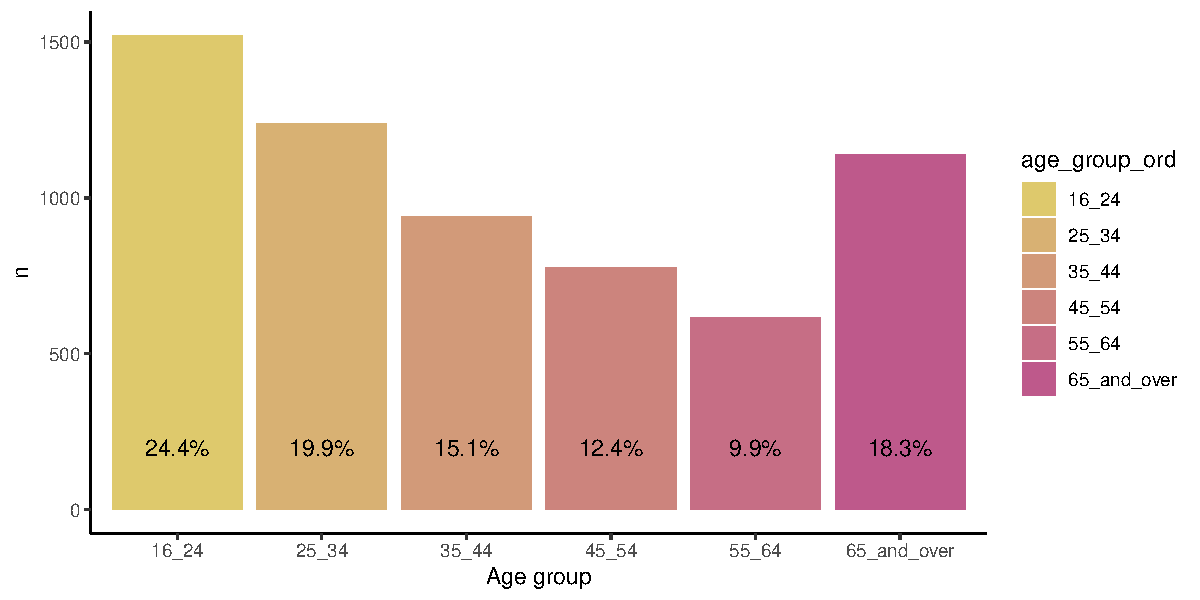
\includegraphics{appendix_files/figure-pdf/trends-by-age-1.pdf}

}

\caption{Age group distributions from the dataset}

\end{figure}

\hypertarget{income}{%
\section{Income}\label{income}}

Survey respondents answered the question ``What is your household annual
income?''. To compare the distribution of responses to this question
from the survey and the Census data, we used the ``Household total
income groups in 2015 for private households'' from the Census data
(available in the Census Data for Ontario website
\href{https://www12.statcan.gc.ca/census-recensement/2016/dp-pd/prof/details/page.cfm?Lang=E\&Geo1=PR\&Code1=35\&Geo2=PR\&Code2=01\&SearchText=Ontario\&SearchType=Begins\&SearchPR=01\&B1=Income\&TABID=1\&type=1}{link}).

\begin{longtable}[]{@{}lll@{}}
\caption{Income percentages from the 2016 Census for
Ontario}\tabularnewline
\toprule\noalign{}
Household income range (CAD) & Percentage & Population Totals \\
\midrule\noalign{}
\endfirsthead
\toprule\noalign{}
Household income range (CAD) & Percentage & Population Totals \\
\midrule\noalign{}
\endhead
\bottomrule\noalign{}
\endlastfoot
\textless{} 15,000 & 5.7\% & 294643 \\
15,000 - 24,999 & 7.5\% & 387688 \\
25,000 - 39,999 & 11.6\% & 599624 \\
40,000- 59,999 & 15.4\% & 796052 \\
60,000 - 89,999 & 19.5\% & 1007988 \\
\textgreater90,000 & 40.3\% & 2083176 \\
\end{longtable}

One difference that is noticeable is that the brackets for income in the
census data are different than the brackets used in the survey. The
census does CAD 4,999 brackets (e.g., CAD 5,000- CAD 9,9999) up to CAD
49,999, followed by CAD 9,999 brackets up to CAD 99,999. After that, the
brackets increase to CAD 24,999, and therefore, it is not possible to
obtain percentages for the 90,000-109,999 and \textgreater110,000
brackets from the survey.

Therefore, in the following code chunk, we created an additional
category for income in the dataset that matched the information from the
Census, and barplots to visualize the proportion of each income bracket
in the dataset.

\begin{figure}

{\centering 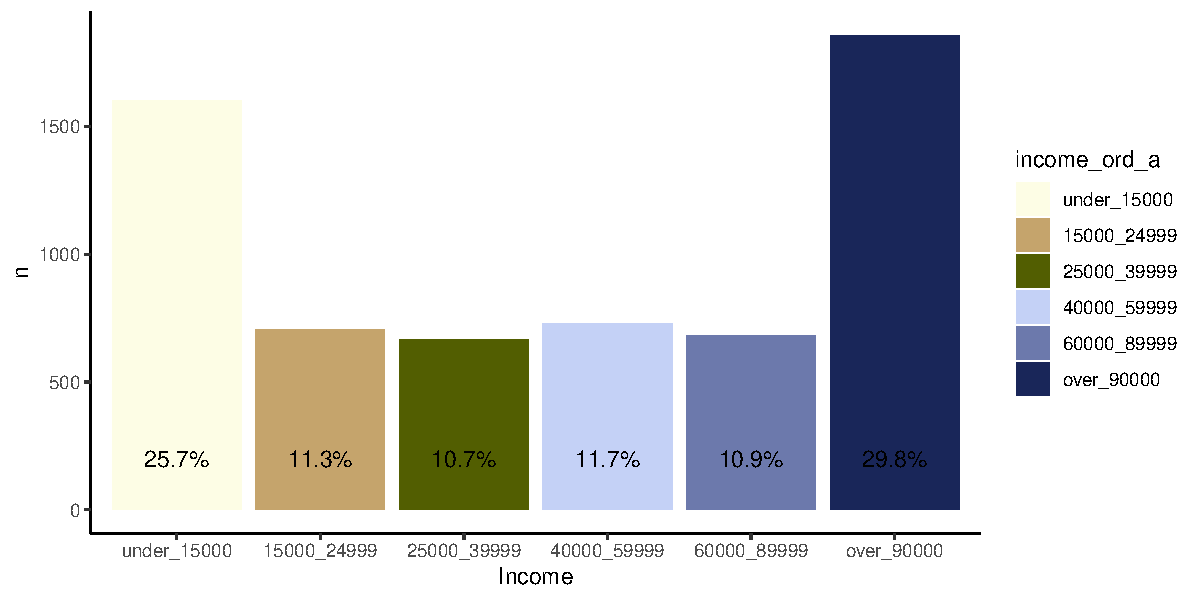
\includegraphics{appendix_files/figure-pdf/income-1.pdf}

}

\caption{Income bracket distribution in the dataset}

\end{figure}

We identified differences again between the survey data and the Census
data. For example, the \textless15,000 bracket accounts for about 24\%
of the responses, a much higher rate than the proportion from the Census
(5.7\%). The other brackets were different as well from the Census data.

\hypertarget{health-regions-population}{%
\section{Health Regions Population}\label{health-regions-population}}

Finally, we obtained population totals for each of the Health Regions
included in the dataset from the Ontario Health Business Plan for
2022-2023 (available
\href{https://www.ontariohealth.ca/sites/ontariohealth/files/2022-05/OHBusinessPlan22_23.pdf}{here}).
The population totals are presented in Table~\ref{tbl-health-regions}.

\hypertarget{tbl-health-regions}{}
\begin{longtable}[]{@{}ll@{}}
\caption{\label{tbl-health-regions}Population Totals for the Health
Regions in Ontario}\tabularnewline
\toprule\noalign{}
Health Region & Population Totals \\
\midrule\noalign{}
\endfirsthead
\toprule\noalign{}
Health Region & Population Totals \\
\midrule\noalign{}
\endhead
\bottomrule\noalign{}
\endlastfoot
North East & 232299 \\
North West & 557000 \\
West & 4095589 \\
East & 3742520 \\
Central & 5032410 \\
Toronto & 1440644 \\
\end{longtable}

Note that as indicated in the paper, we excluded observations from the
North East and North West Health Regions, and therefore, the population
totals for these areas were not used in the final analysis.

\hypertarget{corrections}{%
\section{Corrections}\label{corrections}}

We used the iterative proportional fitting procedure (\emph{raking}) in
order to account for the differences in income, age groups,
race/ethnicity and the population from the Health Regions. Details of
the implementation can be found in the R Script \texttt{raking.R} in the
\texttt{code} directory.

\hypertarget{complete-model-estimates}{%
\section{Complete Model Estimates}\label{complete-model-estimates}}

The figures below present the complete estimates from the regression
models.

\begin{figure}

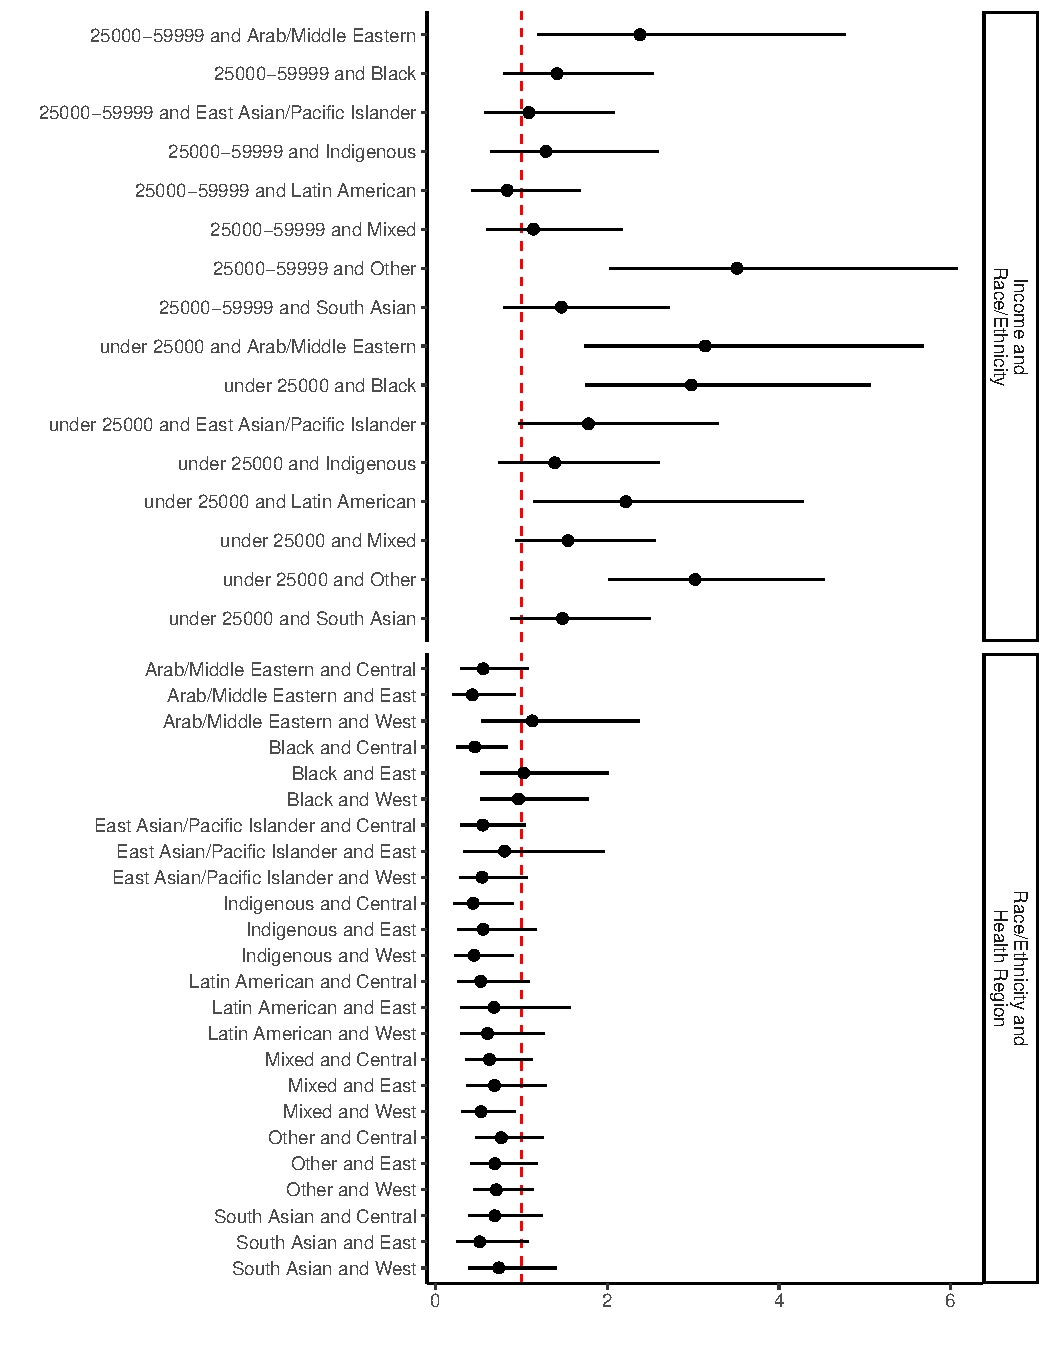
\includegraphics{appendix_files/figure-pdf/fig-model-uncorr-appendix-1.pdf} \hfill{}

\caption{\label{fig-model-uncorr-appendix}Full coefficient estimates and
confidence intervals for the uncorrected model.}

\end{figure}

\FloatBarrier

\begin{figure}

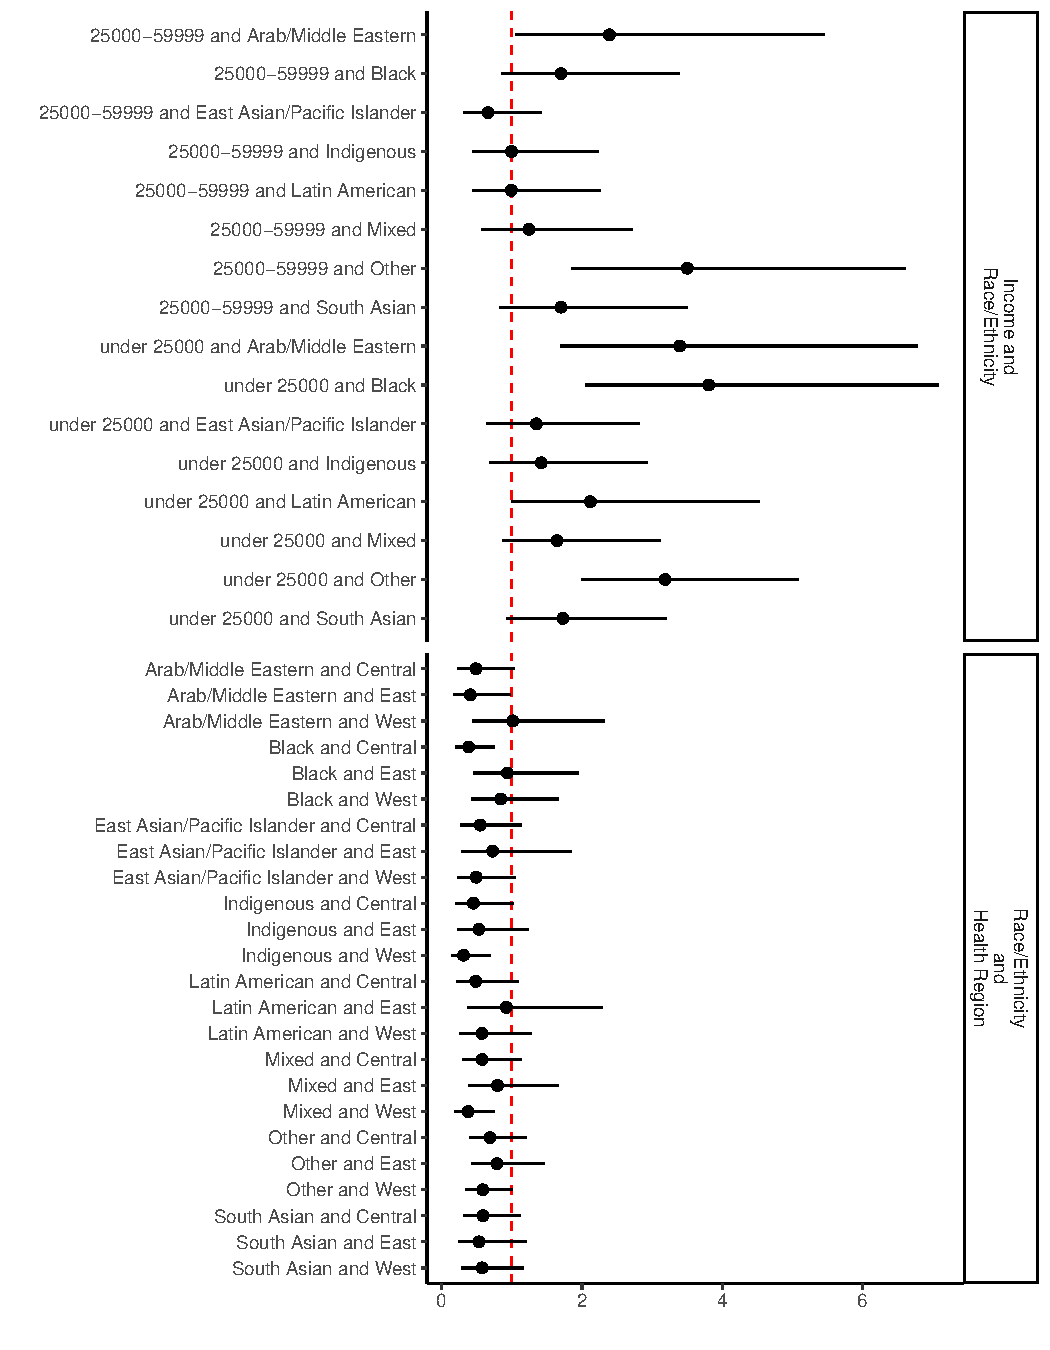
\includegraphics{appendix_files/figure-pdf/fig-model-corr-appendix-1.pdf} \hfill{}

\caption{\label{fig-model-corr-appendix}Full coefficient estimates and
confidence intervals for the corrected model.}

\end{figure}

\FloatBarrier

\hypertarget{interactions-from-the-regression-model}{%
\section{Interactions from the Regression
Model}\label{interactions-from-the-regression-model}}

The plots below show the interactions for Race and Income and Race and
Health Region based on the corrected regression model presented in the
main paper.

\begin{figure}

{\centering 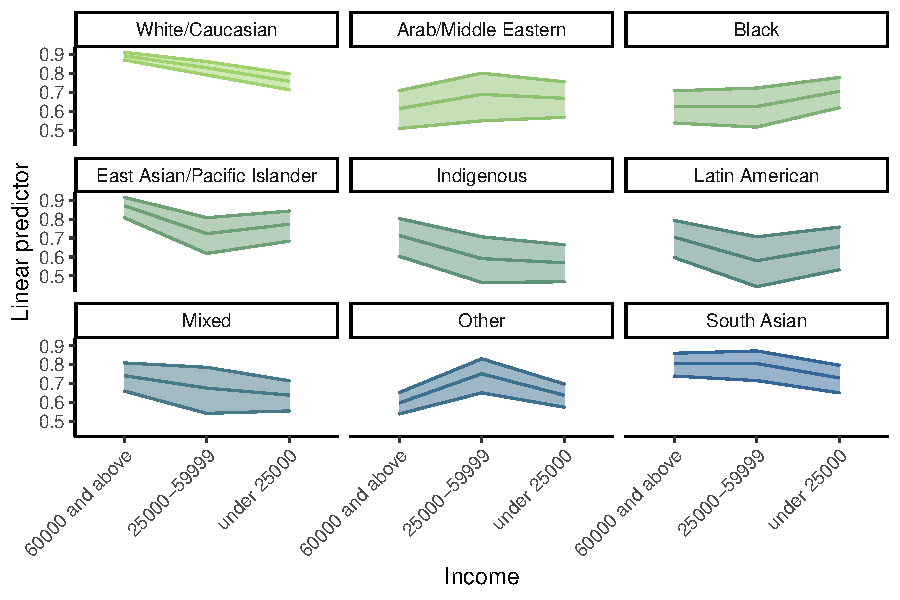
\includegraphics{appendix_files/figure-pdf/interaction-race-income-1.pdf}

}

\caption{Estimated marginal means for the interaction between Race and
Income in the regression model.}

\end{figure}

\begin{figure}

{\centering 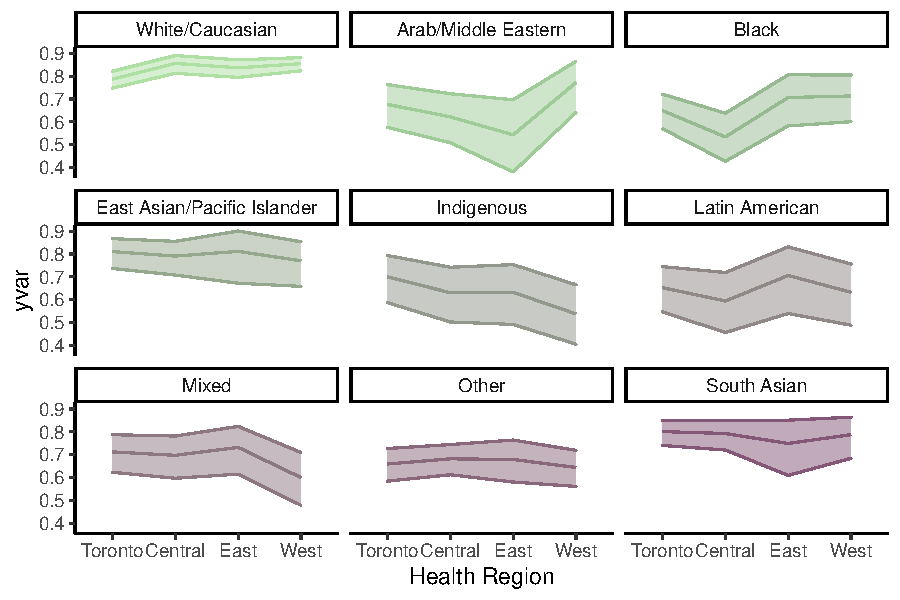
\includegraphics{appendix_files/figure-pdf/interaction-race-hr-1.pdf}

}

\caption{Estimated marginal means for the interaction between Race and
Health Region in the regression model.}

\end{figure}

\hypertarget{socio-economic-information-from-the-survey-data}{%
\section{Socio-economic Information from the Survey
Data}\label{socio-economic-information-from-the-survey-data}}

Tables A-7 and A-8 present summaries of information from the Fields
survey (from the dataset analyzed in the main paper), showing responses
by White/Caucasian individuals by Health Region and proportion of
answers by LHIN in the West Health Region.

\hypertarget{tbl-hr-percentages}{}
\begin{table}
\caption{\label{tbl-hr-percentages}Reported Vaccination Status from the Survey for White/Caucasian
Individuals by Health Region }\tabularnewline

\centering
\begin{tabular}{lcc}
\toprule
\textbf{Characteristic} & \textbf{no}, N = 354 & \textbf{yes}, N = 1,871\\
\midrule
\textbf{Health\_Region} &  & \\
\hspace{1em}West & 105 (15\%) & 582 (85\%)\\
\hspace{1em}Toronto & 127 (19\%) & 533 (81\%)\\
\hspace{1em}East & 66 (14\%) & 396 (86\%)\\
\hspace{1em}Central & 56 (13\%) & 360 (87\%)\\
\bottomrule
\multicolumn{3}{l}{\rule{0pt}{1em}\textsuperscript{1} n (\%)}\\
\end{tabular}
\end{table}

\hypertarget{tbl-west-hr-lhin}{}
\begin{table}
\caption{\label{tbl-west-hr-lhin}Proportion of answers by LHIN (West Health Region) }\tabularnewline

\centering
\begin{tabular}{lc}
\toprule
\textbf{Characteristic} & \textbf{N = 1,460}\\
\midrule
\textbf{LHIN} & \\
\hspace{1em}Hamilton Niagara Haldimand Brant (Hnhb) & 470 (32\%)\\
\hspace{1em}Waterloo Wellington & 400 (27\%)\\
\hspace{1em}South West & 345 (24\%)\\
\hspace{1em}Erie St. Clair & 245 (17\%)\\
\bottomrule
\multicolumn{2}{l}{\rule{0pt}{1em}\textsuperscript{1} n (\%)}\\
\end{tabular}
\end{table}

\hypertarget{tbl-west-region-indigenous}{}
\begin{table}
\caption{\label{tbl-west-region-indigenous}Proportion of answers by LHIN in the West Health Region for Indigenous
Individuals }\tabularnewline

\centering
\begin{tabular}{lcc}
\toprule
\textbf{Characteristic} & \textbf{no}, N = 32 & \textbf{yes}, N = 42\\
\midrule
\textbf{LHIN} &  & \\
\hspace{1em}Hamilton Niagara Haldimand Brant (Hnhb) & 19 (59\%) & 9 (21\%)\\
\hspace{1em}South West & 4 (13\%) & 18 (43\%)\\
\hspace{1em}Waterloo Wellington & 7 (22\%) & 11 (26\%)\\
\hspace{1em}Erie St. Clair & 2 (6.3\%) & 4 (9.5\%)\\
\bottomrule
\multicolumn{3}{l}{\rule{0pt}{1em}\textsuperscript{1} n (\%)}\\
\end{tabular}
\end{table}

\hypertarget{tbl-west-region-mixed}{}
\begin{table}
\caption{\label{tbl-west-region-mixed}Proportion of answers by LHIN in the West Health Region for Mixed
Individuals }\tabularnewline

\centering
\begin{tabular}{lcc}
\toprule
\textbf{Characteristic} & \textbf{no}, N = 41 & \textbf{yes}, N = 76\\
\midrule
\textbf{LHIN} &  & \\
\hspace{1em}Waterloo Wellington & 14 (34\%) & 20 (26\%)\\
\hspace{1em}Hamilton Niagara Haldimand Brant (Hnhb) & 10 (24\%) & 22 (29\%)\\
\hspace{1em}South West & 11 (27\%) & 20 (26\%)\\
\hspace{1em}Erie St. Clair & 6 (15\%) & 14 (18\%)\\
\bottomrule
\multicolumn{3}{l}{\rule{0pt}{1em}\textsuperscript{1} n (\%)}\\
\end{tabular}
\end{table}

\hypertarget{tbl-East-region-Arab}{}
\begin{table}
\caption{\label{tbl-East-region-Arab}Proportion of answers by LHIN in the East Health Region for Arab/Middle
Eastern Individuals }\tabularnewline

\centering
\begin{tabular}{lcc}
\toprule
\textbf{Characteristic} & \textbf{no}, N = 19,716 & \textbf{yes}, N = 23,499\\
\midrule
\textbf{LHIN} &  & \\
\hspace{1em}Toronto \hspace{1em}Central & 0 (0\%) & 0 (0\%)\\
\hspace{1em}Champlain & 13,173 (67\%) & 19,825 (84\%)\\
\hspace{1em}Mississauga Halton & 0 (0\%) & 0 (0\%)\\
\hspace{1em}Hamilton Niagara Haldimand Brant (Hnhb) & 0 (0\%) & 0 (0\%)\\
Central & 0 (0\%) & 0 (0\%)\\
\hspace{1em}Waterloo Wellington & 0 (0\%) & 0 (0\%)\\
\hspace{1em}Central West & 0 (0\%) & 0 (0\%)\\
\hspace{1em}South West & 0 (0\%) & 0 (0\%)\\
\hspace{1em}Central East & 6,543 (33\%) & 3,674 (16\%)\\
\hspace{1em}Erie St. Clair & 0 (0\%) & 0 (0\%)\\
\hspace{1em}North Simcoe Muskoka & 0 (0\%) & 0 (0\%)\\
\hspace{1em}South East & 0 (0\%) & 0 (0\%)\\
\bottomrule
\multicolumn{3}{l}{\rule{0pt}{1em}\textsuperscript{1} n (\%)}\\
\end{tabular}
\end{table}



\end{document}
